\chapter{Results \& Discussion}
\section{Introduction}

\section{Model Analysis} \label{analysis}
Given the overall adoption trends, some elements need further discussion. A few key parameters embedded in the model require further analysis. To understand their role in the model, a sensitivity analysis will be performed of these parameters. This sensitivity analysis will be performed for the loss aversion and battery subsidies\footnote{Since the author was constrained by the size of this Thesis, the discussion of the residual load and network charge could not be included in the report but can be found on: }.
\subsection{Residual load}
Since the utility death spiral depends on the amount of revenue changes the DSO has to recuperate when a portion of its customers start adopting DER, the residual load of the environment will be the driving force behind this utility death spiral. The higher the residual load as a fraction of the total load, the more recurring revenue the DSO can rely on. This will make it easier for the DSO to pay for all the costs he must incur to maintain and upgrade his infrastructure. A lower residual load, however, will force the DSO to increase his tariffs more to maintain his revenue. The extent of a difference in residual load will be discussed in the subsequent paragraphs. Besides the standard residual load case, where $Resid.\: load = Repl. \:load$, two additional scenarios will be tested. The first one will be for a lower residual load ($Resid. \: load = 0.33*(Repl.\: load)$) and a higher residual load  ($Resid. \: load = 3*(Repl. \: load)$)
\newline \newline \noindent
The PV adoption for different residual load cases can be found in Figure \ref{Figure:pvresid}. 
\begin{figure}[h!]
\centering
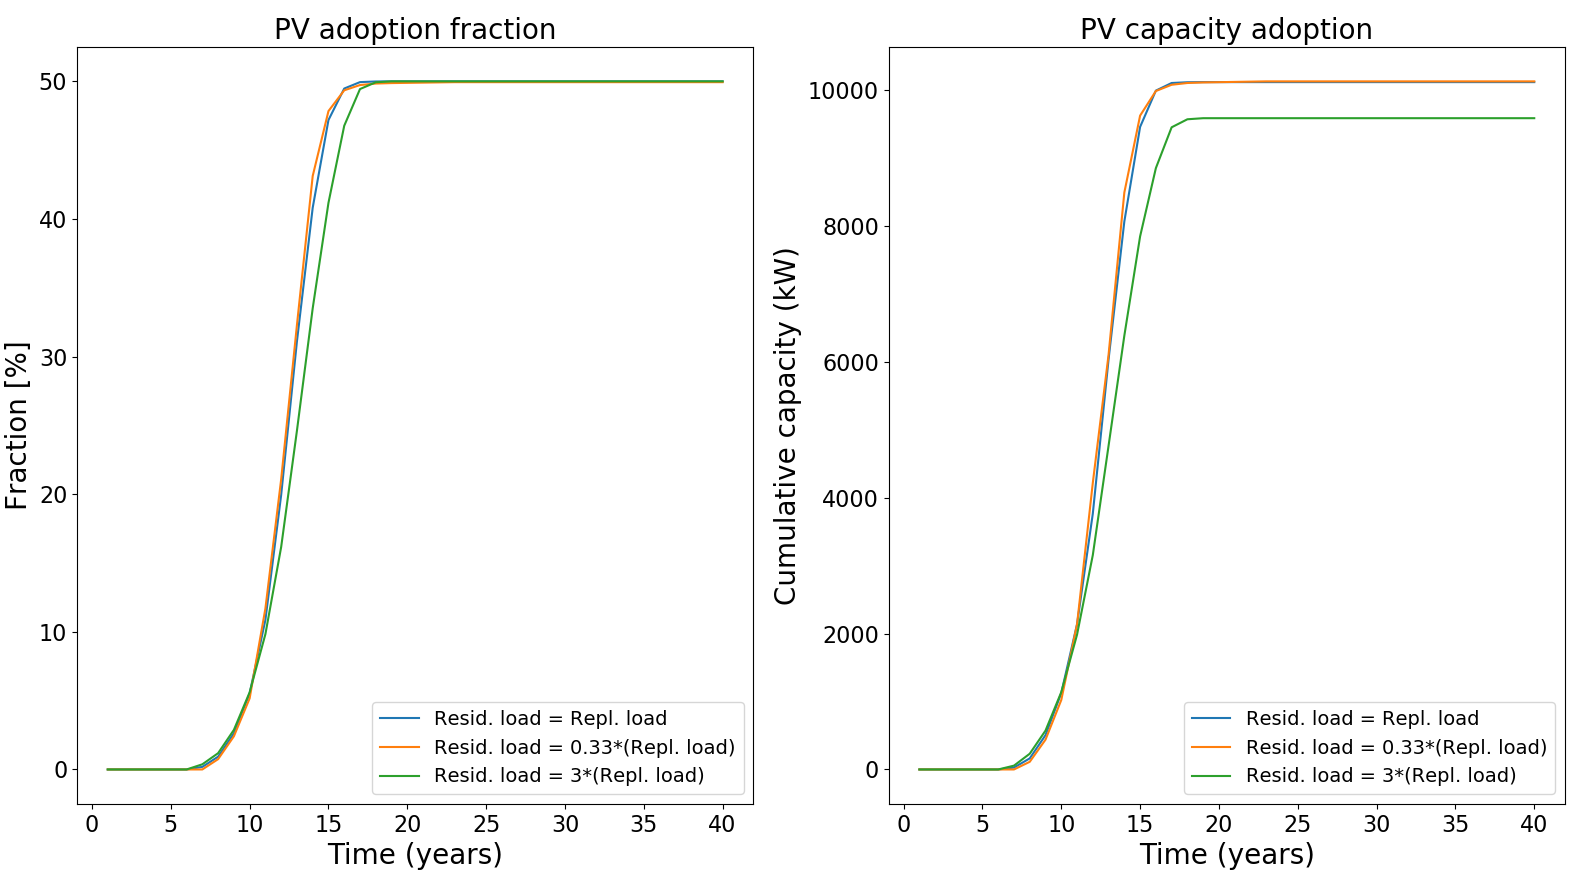
\includegraphics[width=12cm]{ModelAnalysis/PVresid.png}
\caption{PV adoption for different residual loads}
\label{Figure:pvresid}
\end{figure}
 \noindent
Here, the effect of different residual loads is quite subtle. The results for the three residual loads are quite similar, both in adoption fraction and in cumulative PV capacity adopted. The only exception is the cumulative PV capacity for the higher residual load, which will be slightly lower due to the lower savings. This also applies to the battery technology, although the cumulative capacity does show some more variation, as can be seen in Figure \ref{Figure:batresid}. For both technologies, the cumulative adopted capacity for the higher residual load will be lower since the savings will be lower. These savings will be lower because the DSO will have less recurring revenue to rely on, which will force him to adapt his tariffs more rapidly. For the higher residual load, the opposite effects will play. 
\begin{figure}[h!]
\centering
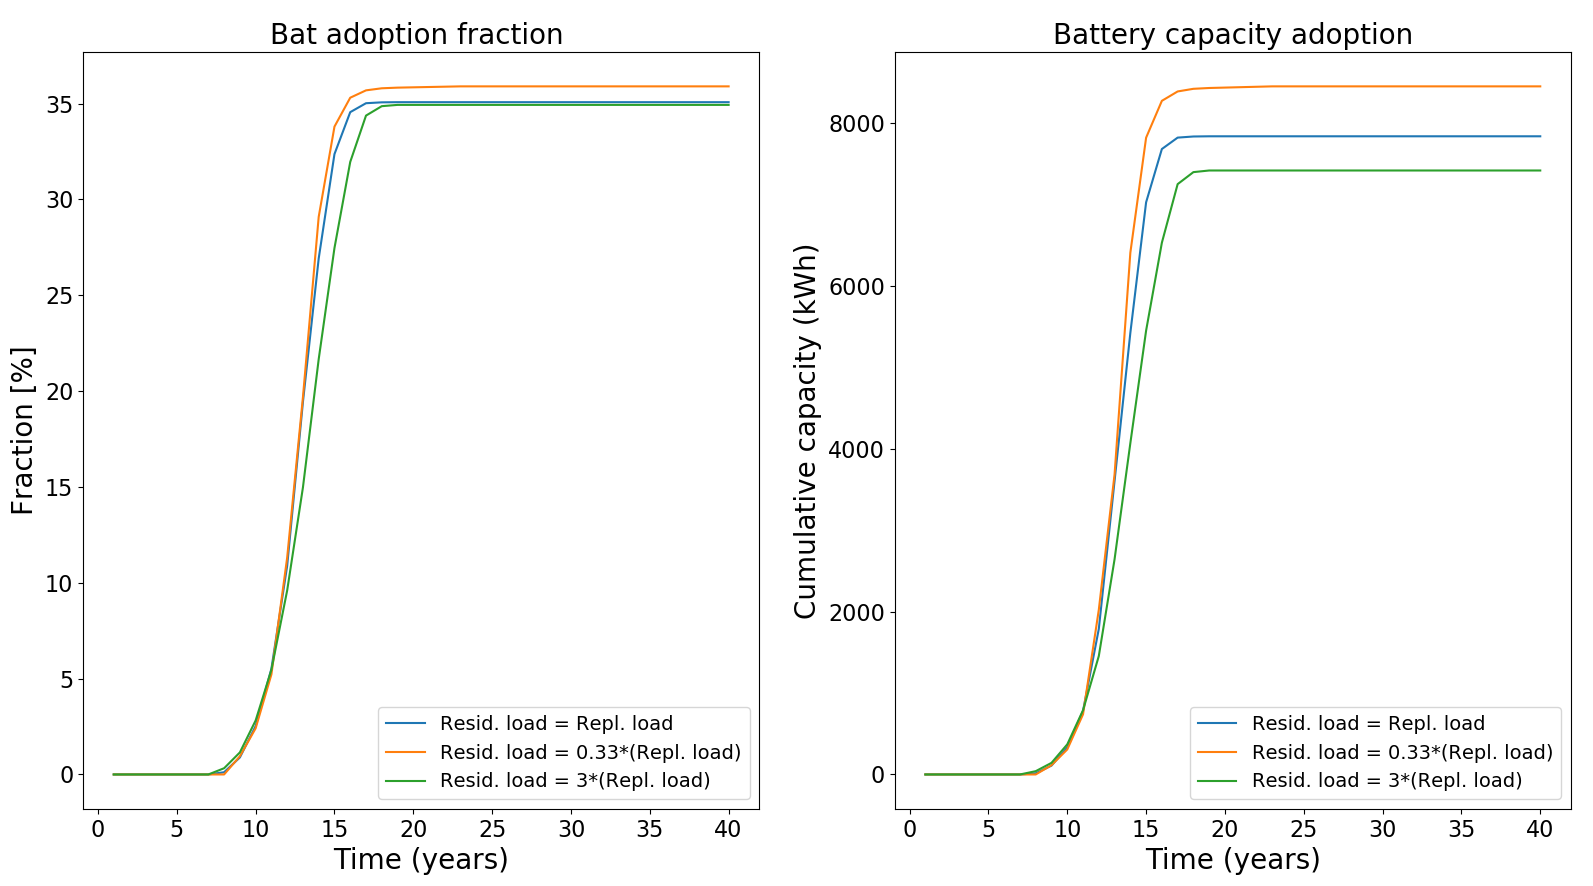
\includegraphics[width=12cm]{ModelAnalysis/BatResid.png}
\caption{Battery adoption for different residual loads}
\label{Figure:batresid}
\end{figure}
\noindent
The resulting configuration distribution can be seen in Figure \ref{Figure:configresid}. Here, the effect of different residual loads becomes more visible. For the lower residual loads, which translates into higher tariffs and savings, the largest configuration (4\textit{kW}/5\textit{kWh}) will become more popular. For the higher residual load, the tariffs and savings will be lower, making this configuration less popular. In fact, the change in battery adoption that can be seen in Figure \ref{Figure:batresid} is mainly due to the variation of this 5\textit{kWh} configuration.
In addition to the largest configuration, the variation of the residual load will also have an effect on smaller configurations, most notably the 1.5\textit{kW}/2\textit{kWh} installation. Contrary to the larger configurations, this one will become more popular in the high residual load case, when savings are lower, while being less popular in the low residual load case, when savings are higher. The resulting distribution tariff can be found in Figure \ref{Figure:distresid}. In parallel with the adoption levels, the distribution tariff will increase by more than 300\% in the low residual load case, while this increase will only be 33.1\% in the case of a higher residual load. 
\begin{figure}[h!]
\centering
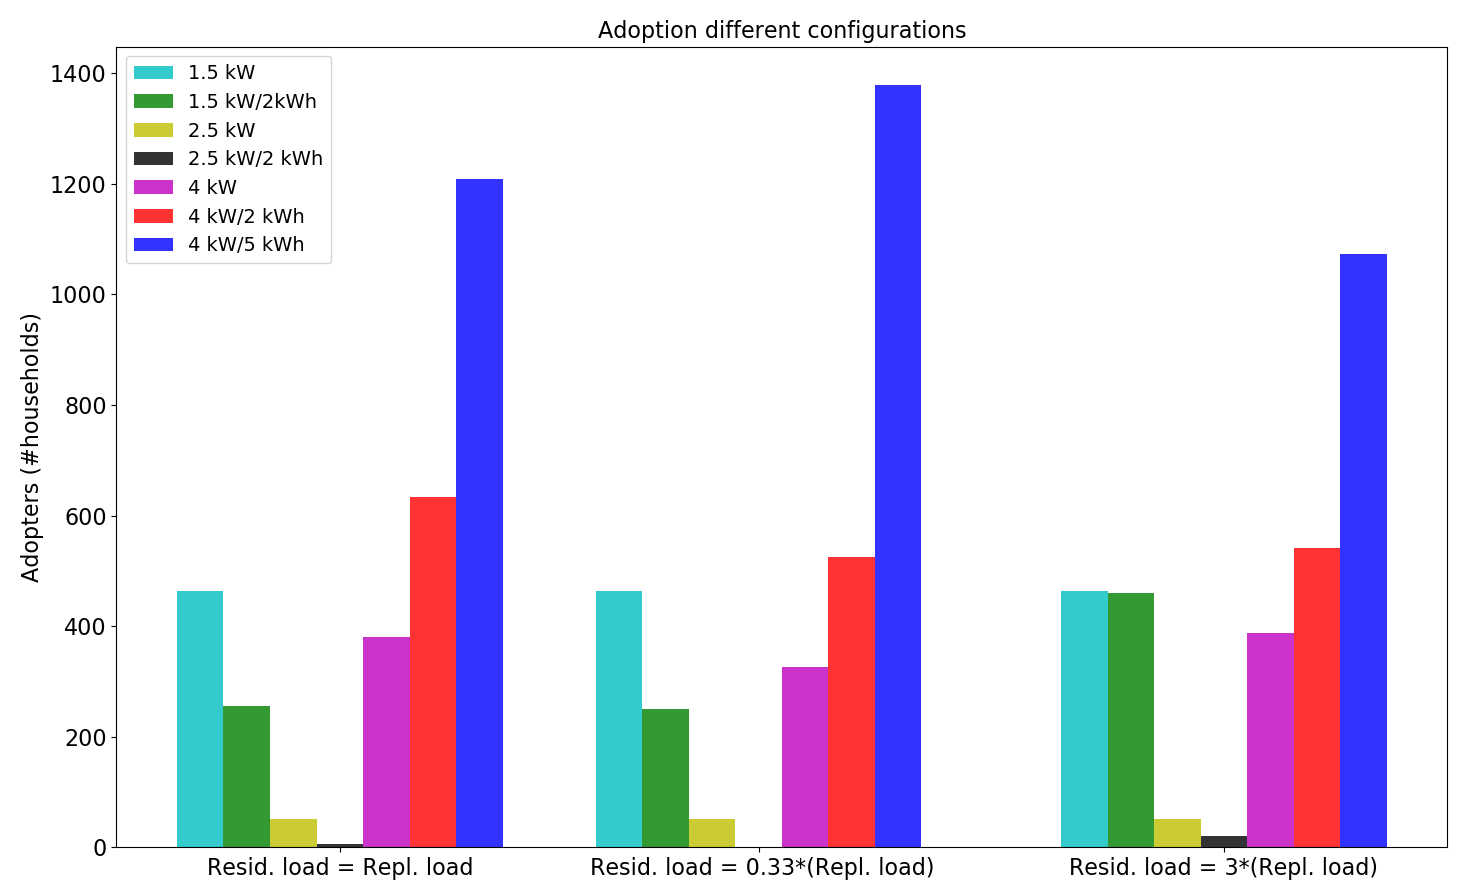
\includegraphics[width=12cm]{ModelAnalysis/ConfigResid.png}
\caption{Configurations for different residual loads}
\label{Figure:configresid}
\end{figure}
\noindent
The resulting configuration distribution can be seen in Figure \ref{Figure:configresid}. Here, the effect of different residual loads becomes more visible. For the lower residual loads, which translates into higher tariffs and savings, the largest configuration (4\textit{kW}/5\textit{kWh}) will become more popular. For the higher residual load, the tariffs and savings will be lower, making this configuration less popular. In fact, the change in battery adoption that can be seen in Figure \ref{Figure:batresid} is mainly due to the variation of this 5\textit{kWh} configuration.
In addition to the largest configuration, the variation of the residual load will also have an effect on smaller configurations, most notably the 1.5\textit{kW}/2\textit{kWh} installation. Contrary to the larger configurations, this one will become more popular in the high residual load case, when savings are lower, while being less popular in the low residual load case, when savings are higher. The resulting distribution tariff can be found in Figure \ref{Figure:distresid}. In parallel with the adoption levels, the distribution tariff will increase by more than 300\% in the low residual load case, while this increase will only be 33.1\% in the case of a higher residual load. 
\newline \newline \noindent
The resulting distribution tariff can be found in Figure \ref{Figure:distresid}. In parallel with the adoption levels, the distribution tariff will increase by more than 300\% in the low residual load case, while this increase will only be 33.1\% in the case of a higher residual load.  
\begin{figure}[h!]
\centering
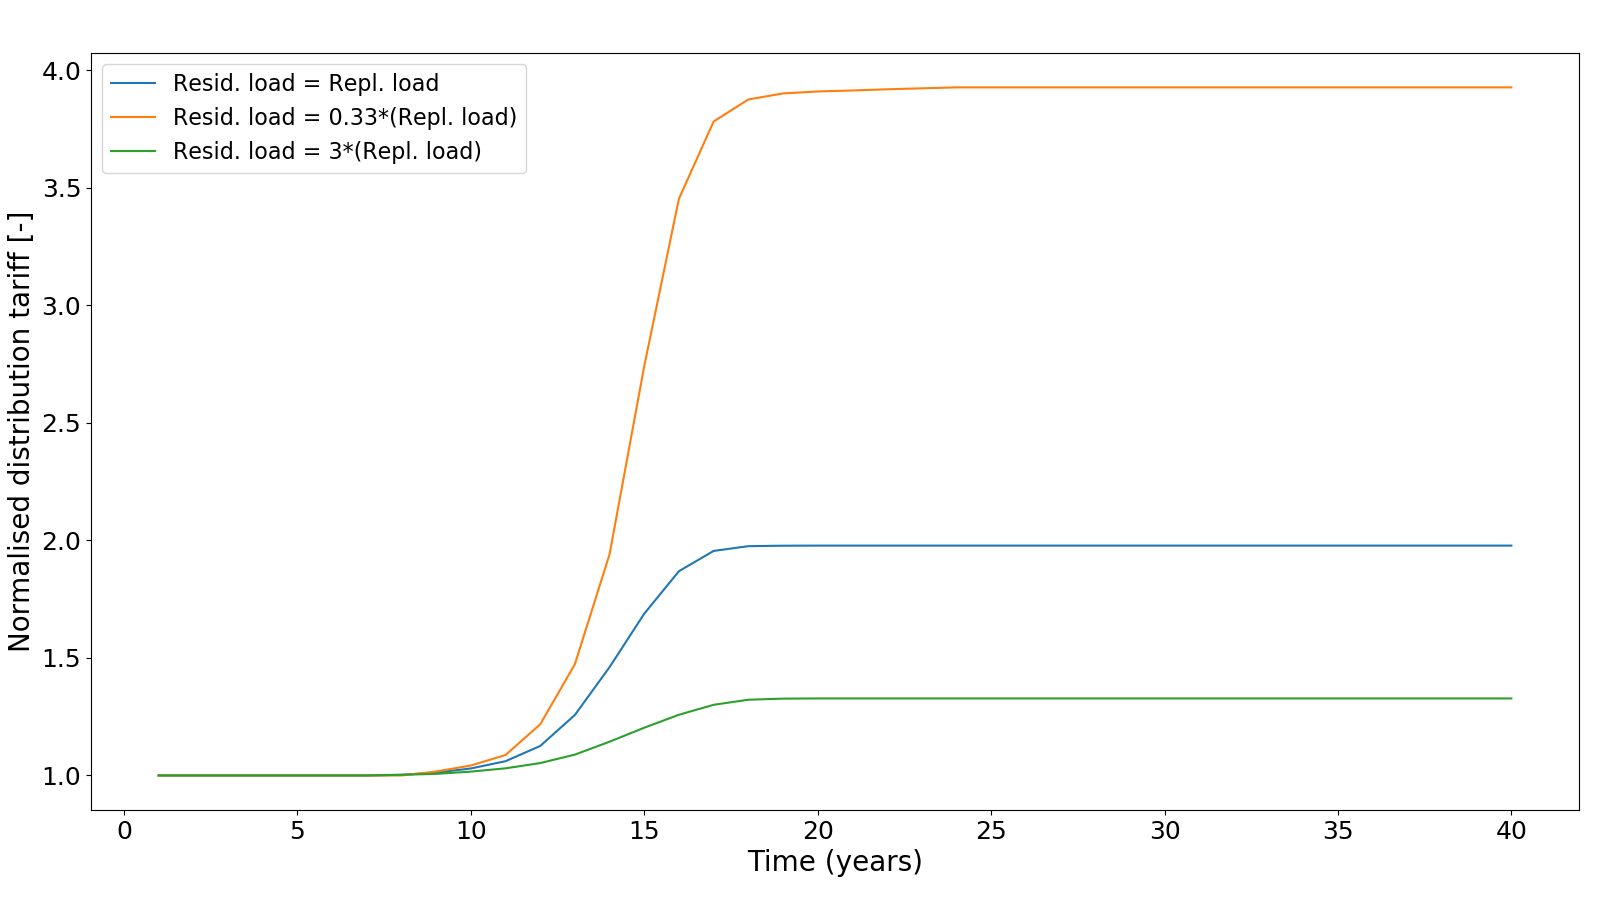
\includegraphics[width=10cm]{ModelAnalysis/distresid.png}
\caption{Distribution tariff for different residual loads}
\label{Figure:distresid}
\end{figure}
\noindent
Judging by the data presented in this section, the residual load has an effect on the adoption of certain configurations. Most notably, the adoption of the 1.5\textit{kW}/2\textit{kWh} and 4\textit{kW}/5\textit{kWh} configurations will change as a function of the residual load. This is mainly due to the effect of a change in the network charge on the savings. The lower the residual load, the more popular the large configurations and the less popular the small configurations will be. The higher the residual load, the more popular the smaller configurations are and the less popular the larger configurations. This adoption shift between different configurations will cause the effect on the aggregate adoption fraction and capacity adopted to be rather limited, with the exception of the battery capacity adopted. In parallel with the DER evolution, the network charges will increase in the utility death spiral process. 
\subsection{Network charge}
\label{distanal} As was already discussed in Section \ref{compar}, the different network charges have a different effect on the savings and, therefore, the overall adoption and subsequent utility death spiral. The main driver for this difference in adoption between the net volumetric tariff and annual capacity offtake tariff is the difference in savings between the two tariffs. Both the way in which savings are created as well as the effect of this change in savings on the adoption of DER will be discussed in the next few paragraphs.
\newline \newline \noindent
Since the savings for a household due to the adoption of DER consist of both energy costs and (some) distribution costs, the overall savings will evolve with these components. In the case of the net volumetric distribution tariff, the distribution component can be calculated using Equation \ref{distnet}. This cost formula suggest that the savings of the household can increase substantially in case $q_{net}$ reaches a value close to zero. As can be seen in Figure \ref{Figure:netdem}, $q_{net}$  of all but two configurations is equal to zero, meaning that all distribution charges are avoided. Compared to $q_{net}$ for no DER adoption, the savings of the distribution component and by extension the electricity cost are significant. 
\begin{figure}[h!]
\centering
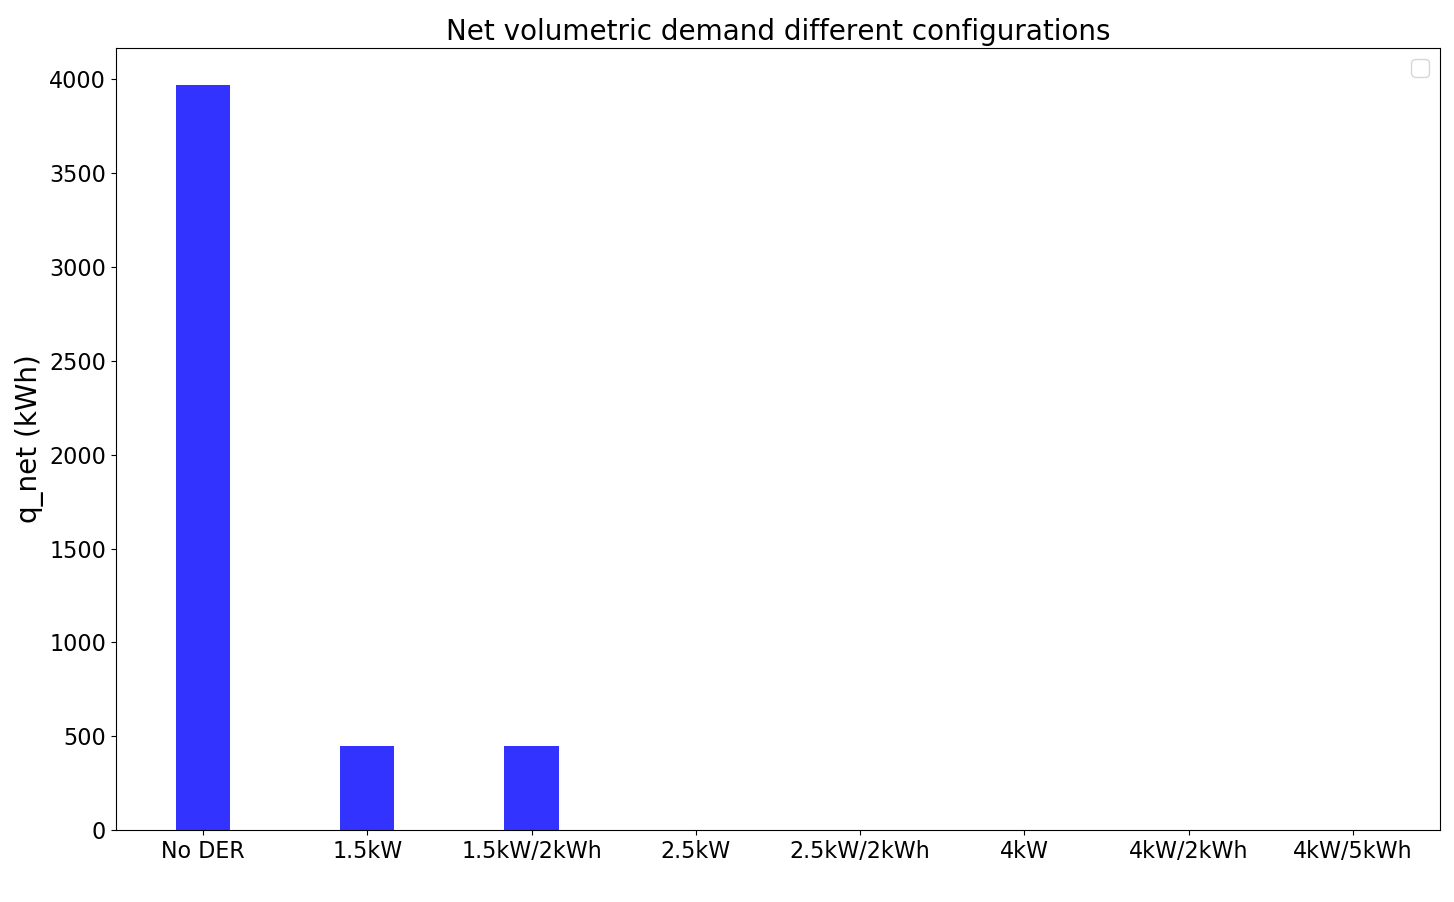
\includegraphics[width=12cm]{ModelAnalysis/Netdemand.%png}
\caption{Net volumetric demand for different DERs %configurations}
\label{Figure:netdem}
\end{figure}
\noindent
For the annual capacity offtake tariff, the distribution cost can computed using Equation \ref{qcap}. This network charge formulation suggests that, like in the volumetric case, the distribution cost could decrease to zero. When looking at Figure \ref{Figure:peakdem}, however, it becomes clear that $q_{cap}$ and the distribution cost component will remain strictly positive for all configurations.  
\begin{figure}[h!]
\centering
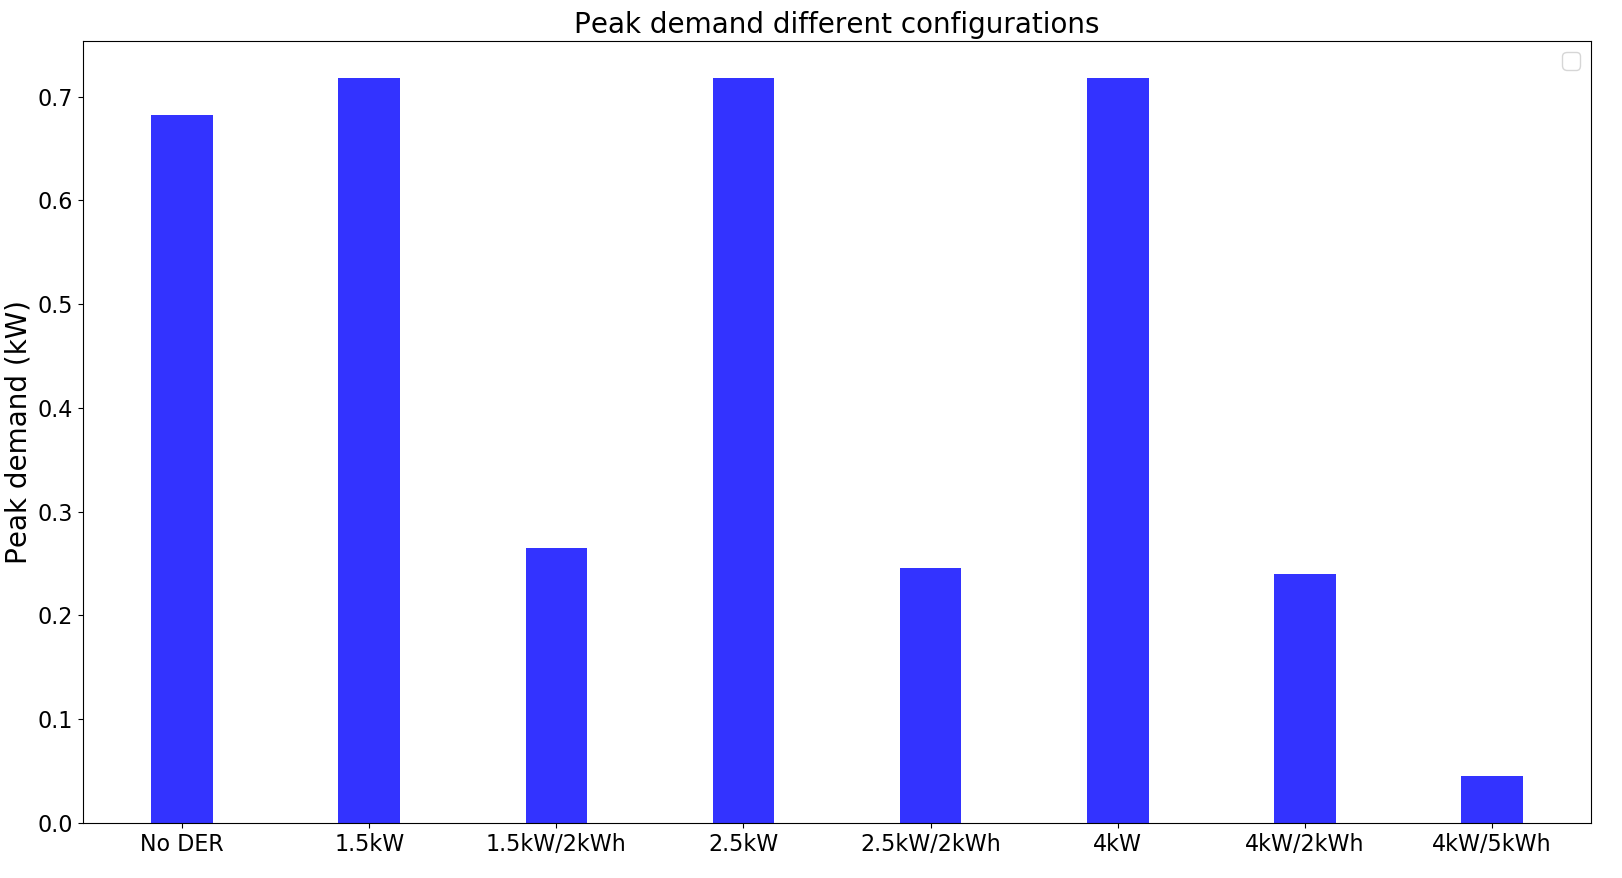
\includegraphics[width=12cm]{ModelAnalysis/PeakDemand.png}
\caption{Different peak demands}
\label{Figure:peakdem}
\end{figure}
\noindent
Due to the previously discussed difference in distribution cost for the two different network charges, the savings will de different, as can be seen in Figure \ref{Figure:Savings} \footnote{The represented data is the average of the savings for all configurations}. Here, it can be seen how the savings realised in the case of the net volumetric distribution tariff are much higher than for the annual capacity offtake tariff. Besides having a larger initial value, the savings for the volumetric network charge also increase more streadily than those in the capacity tariff case: the volumetric savings increase by 39.6\% throughout 40 year simulation, whereas they only increase by 6.8\% in the capacity case pver the same period. This is a direct result of the higher initial value in the volumetric distribution tariff case: the higher savings cause a higher adoption incentive, causing the utility death spiral to manifest itself more clearly, which will cause the distribution tariff to increase further. The results discussed in Section \ref{compar} showed the extent of this utility death spiral for the different policies. 
\begin{figure}[h!]
\centering
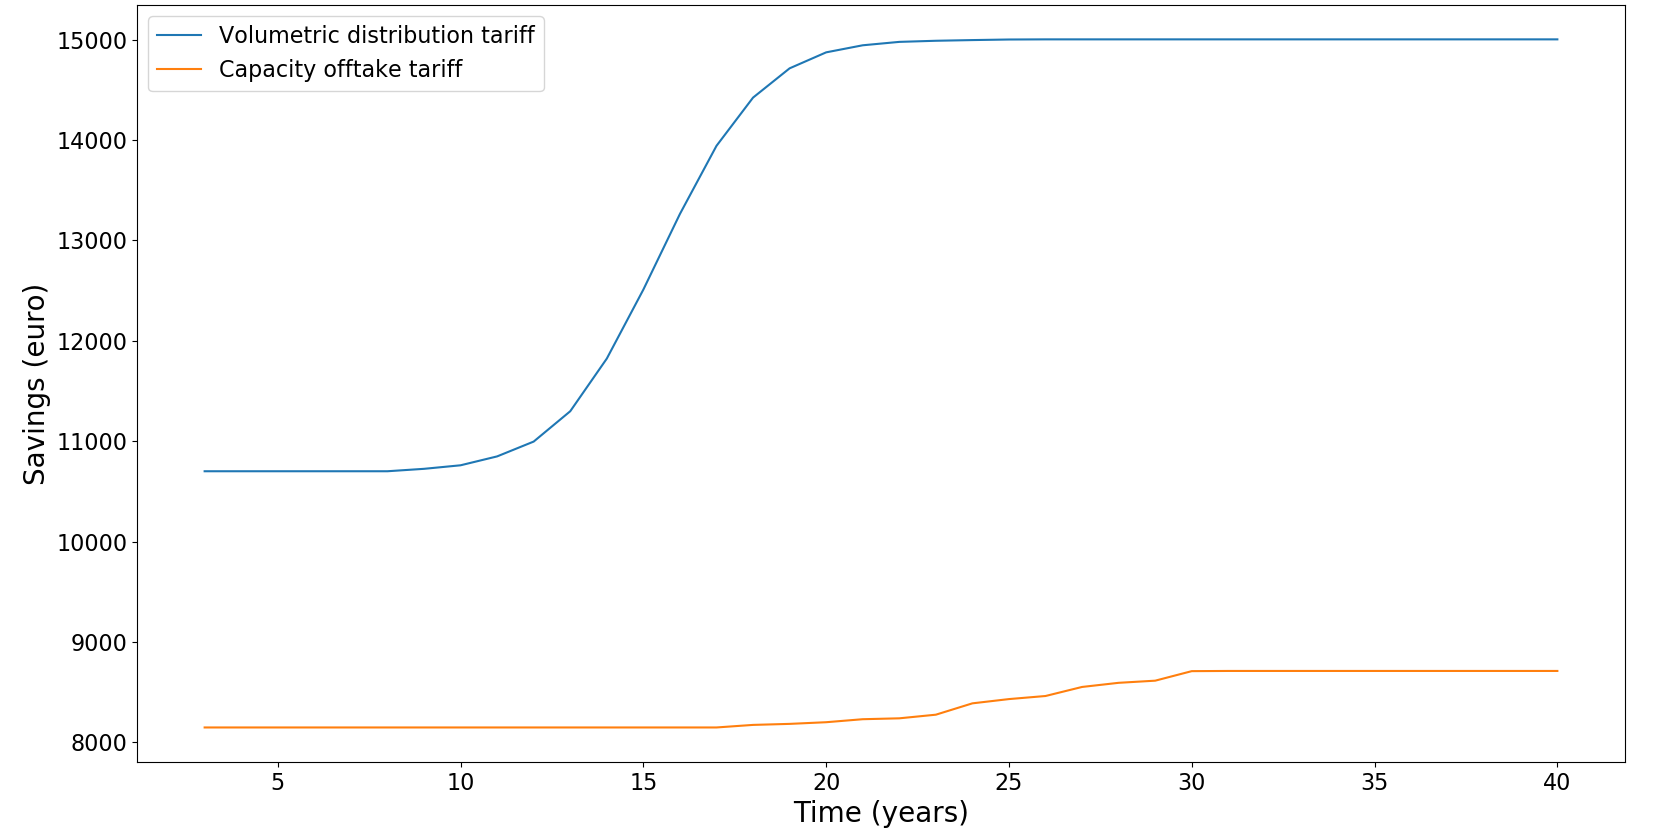
\includegraphics[width=12cm]{ModelAnalysis/Savings.png}
\caption{Savings for the volumetric and capacity tariff}
\label{Figure:Savings}
\end{figure}
\subsection{Preliminary analysis \& Conclusion}
What also became clear from this analysis, is the role of the residual load in the DER adoption process. Since a lower residual load causes the network charges and savings to be higher, the incentive to adopt DER becomes higher, thereby reinforcing the network charge increase once again, creating a vicious circle. Currently, the fraction of DER in the overall electricity landscape still is limited, but rising quickly. Over the next few decades, as policy makers intend to make a large portion of the households adopt DER to reduce emissions, the residual load will become a smaller portion of the overall load, which would cause the utility death spiral effects to be amplified. The distribution cost evolution for low residual loads that was presented in Figure \ref{Figure:distresid} could, therefore, materialize over the next few decades if appropriate action is not taken. As was discussed in Section \ref{compar}, the capacity-based network charge can mitigate these effects. The main reason for this, as was discussed in Section \ref{distanal}, is the change in the distribution cost component and its effects on the savings and adoption incentive. For the net volumetric distribution tariff, this cost component decreases to zero for most configurations, generating more savings to the households and encouraging DER adoption. The design of the capacity offtake tariff, however, will cause the distribution component to decrease by a smaller amount for most configurations, generating less savings to the households, thereby encouraging DER adoption to a lesser extent. 
